\documentclass[11pt, oneside, halfparskip, smallheadings, automark]{scrreprt}

\usepackage[utf8]{inputenc}
\usepackage[T1]{fontenc}
\usepackage[ngerman]{babel}
\usepackage{palatino}

% Weiter Pakete können hinzugefügt werden
\usepackage{
  booktabs,
  graphicx,
  xcolor
}



%%  Für klickbare Inhaltsverzeichnise, Verweise etc.
\usepackage[
  bookmarks=true,           % Lesezeichen erzeugen
  bookmarksopen=true,
	colorlinks=true,
	linkcolor=black, 
	anchorcolor=black, 
	citecolor=black, 
	filecolor=black, 
	menucolor=black, 
	pagecolor=black,
	urlcolor=black
]{hyperref}

%%  Abkürzungsverzeichnis
\usepackage[
     footnote,
     nohyperlinks
]{acronym}

%% Neue Makros
\newcommand{\infoprojekt}{Informatikprojekt Klasse 10}

%% Seiten- und Layouteinstellung
\usepackage[left=3.3cm,%
            top=3cm,%
            bottom=3cm,%
            textwidth=15.5cm,%
            marginparwidth=0cm]{geometry}

\usepackage{setspace}
\onehalfspacing					%%  1,5 zeilig

 
%% Für Bildunterschriften etc.
\usepackage{array}
\usepackage[font=small, labelfont=scriptsize,sf,textfont=it]{caption}      

%% Kopf- und Fußzeilen
\usepackage{scrpage2}
\clearscrheadings
\clearscrplain
\pagestyle{scrheadings}
\rohead{\rightmark}
\rofoot[\pagemark]{\pagemark}
\setheadsepline{.4pt} % Linie unter dem Head

%% Fussnoten bündig
\deffootnote{1.2em}{0em}{%
            \makebox[1.2em][l]{\bfseries\thefootnotemark}}


%   ********************************************************************************
%
%        Anpassen, oder entwerfen einer eigenen Titelseite

\title{Entwicklung einer Website zur Verwaltung der Korrespondenzzirkel}
\author{Elea Kurschel \\ Celine Suchanek}

\subject{\infoprojekt}
\publishers{\emph{Betreuer:} \\Herr Stephen Mehlhos\\Herr Mirko König}

%
%   ********************************************************************************


\usepackage{blindtext}
\begin{document}

\maketitle

\tableofcontents


%%  Abkürzungsverzeichnis

\chapter*{Abkürzungsverzeichnis}

\begin{acronym}
 %\acro
\end{acronym}
\chapter{Einleitung}
Das Carl-Zeiss-Gymnasium Jena bietet für mathematisch-naturwissenschaftlich interessierte und begabte Schüler im Raum Ostthüringen verschiedene Korrespondenzzirkel an. Das Ziel dabei ist es, die optimale Ausprägung und Weiterentwicklung der Schülerpersönlichkeit und ihrer spezifischen Fähigkeiten und  Fertigkeiten über den Unterricht hinaus mit anspruchsvollen Aufgaben, erstellt von Lehrern mit langjähriger Erfahrung. Bisher wurden die Teilnahme und die Auswertung  manuell mit Hilfe von verschiedensten Excel-Tabelle gemacht. Mit unserem Projekt möchten wir das ganze über eine zentrale Datenbank vereinfachen und realisieren. Die Verwaltung soll über eine Website gestaltet werden.\\
\\
Einen Großteil des Projektes wird mit Eclipse erarbeitet. Dieses Java-Programm ist eine kostenlose, open source Entwicklungsumgebung zum Entwickeln von anderen Programmen in Java. Wir nutzen es jedoch für PHP. Das Projekt wird unter Windows entwickelt, da Windows auf den verwendeten Geräten verfügbar ist. (MySQL: leistungsfähiges Datenbanksystem, kostenfrei verfügbar.) Außerdem nutzten wir git. Das ist ein Programm zur Quellcodeverwaltung um gemeinsam am Projekt zuarbeiten. Die Daten werden in einem Repository gespeichert. Dazu kommt die Verwendung von github. Auf einer Seite werden die Repositories abgelegt und kann so mit anderen geteilt werden. Tortoise ist eine Benutzeroberfläche um git über Windows einfach nutzen zu können, was für uns die Arbeit wesentlich erleichtert. Die Dokumentation wird mit LaTex erstellt.
\\
XAMPP

\chapter{Theoretische Grundlagen}

Wir möchten Korrespondenzzirkel, Teilnehmer, Aufgaben und Ergebnisse verwalten.

Für jeden Korrespondenzzirkel müssen Fach und Klassenstufe festgelegt werden. 
Teilnehmer sind Schüler, deren Name, Anschrift und Schule eingegeben wurden. Für jede Schule muss der Name und die Anschrift gespeichert werden. 
Jeder Korrespondenzzirkel besteht aus mehreren Aufgabenserien, die jeweils eine maximal erzielbare Punktzahl haben. Eine Aufgliederung auf einzelne Aufgaben soll aus Gründen der Übersichtlichkeit nicht erfolgen.
Für abgegebene Aufgaben bekommen Teilnehmer Punkte. Für jeden Zirkel soll es eine nach Schülern gegliederte Zusammenfassung aller bisher erzielten Punkte geben.

Um mit dem Programm arbeiten zu können, muss man über ein Nutzerkonto verfügen. Die Anlage von Nutzerkonten wird durch einen Administrator geregelt. Dies ist ein spezieller Nutzer mit erweiterten Rechten.

Die Software sollte parallel durch mehrere Nutzer verwendbar sein.
Die Programmierung sollte mit möglichst geringem Aufwand erfolgen.
Da die beiden Programmierer in verschiedenen Orten wohnen, muss die gleichzeitig Arbeit am Projekt koordiniert werden.

\chapter{Lösungsidee}

Die parallele Nutzung ermöglichen wir durch eine Aufbau einer eigenen Webseite. Dadurch müssen die Nutzer auch keine Software auf ihren Rechnern installieren. Die Webseite kann in der Schule auf einem beliebigen Server gehostet werden. 

Als Datenbanksystem verwenden wir MySQL und als Programmiersprache PHP zusammen mit Apache. Für die Entwicklung wird XAMPP eingesetzt, da es die Installation und Verwaltung dieser Softwarepakete unter Windows vereinfacht. Später können MySQL, PHP und Apache auf einem beliebigen Server installiert werden. \cite{Xampp}

Der Zugriff auf das Programm erfolgt mit einem beliebigen Browser. Für eine bessere Benutzerinteraktion wird zum Teil auf JavaScript zurückgegriffen. Damit können Teile des Programms direkt im Browser laufen.

Um die Pflege der Stammdaten der Teilnehmer zu erleichtern, trennen wir die Stammdaten der Schüler von den Teilnahmeinformationen. Damit müssen die Daten von Schülern, die an mehreren Zirkeln teilnehmen, nur einmal eingegeben werden. Bei den Schülern speichern wir zudem anstelle der aktuellen Klassenstufe das Einschulungsjahr. Dadurch wird nach einem Schuljahreswechsel die Klassenstufen automatisch angepasst und die Daten der Schüler können wiederverwendet werden.

Eine komplette Webseite zu programmieren ist sehr aufwändig. Wir nutzen deshalb das PHP-Framework Laravel. Es nimmt dem Entwickler sehr viel Arbeit beim Erstellen einer Website und beim Zugriff auf die Datenbank wird ab. Das Framework verwendet Bootstrap, um die Webseite optisch ansprechend zu gestalten. \cite{Bootstrap} \cite{laravel}

Für die parallele Entwicklung setzen wir die Quellcodeverwaltung git ein. Jeder kann dadurch für sich arbeiten und die Ergebnisse regelmäßig über github austauschen. github sorgt auch dafür, dass das Projekt ausfallsicher gespeichert ist.
\chapter{Programmdokumentation}
\blindtext

\blindtext

\blindtext

\chapter{Programmablaufprotokolle}

Zum Testen wurde folgendes Beispiel ausgewählt:

Nach dem Anmelden drückt man auf "`Schule"' und dort "`Neue Schule anlegen"'. Die neue Schule hat den Namen Musterschule, befindet sich in der Musterstraße 1 in 01234 Musterstadt. Nach dem Eintragen der Daten kann diese gespeichert werden und die neu angelegte Schule erscheint in der Liste. 

Nun ist es möglich bei "`Schüler"' neue Schüler hinzuzufügen. Wir nehmen Erika Musterfrau, Max Mustermann und Viktor Vorbeeld. Erika besucht die 9. Klasse, ebenso Max und Viktor. Alle 3 gehen auf die eben angelegte Musterschule und wohnen in der Mustergasse in 01234 Musterstadt. 

Jetzt ist es möglich, über "`Fächer"' ein neues Fach anzulegen, in unserem Beispiel Biologie. 

Nun kann man zu "`Zirkel"' wechseln und einen neuen im Fach Biologie, Klassenstufe 9 anlegen. Dabei muss man beachten, dass man das richtige Schuljahr eingestellt hat.

Klickt man nun auf "`Teilnehmer verwalten"', werden uns alle Schüler der Klassenstufe 9 angezeigt, also auch unsere Drei aus der Mustergasse. Von diesen drei Schülern wollen aber nur Erika und Viktor am Biologiezirkel teilnehmen, deshalb klickt man bei den beiden auf Eintragen. Sie sind jetzt in dem Zirkel und bekommen Aufgaben zugeschickt. Durch Klicken auf den Zirkelnamen kommt man zurück zur Übersichtseite von dem Zirkel, wo alle beide registrierten Teilnehmer aufgeführt sind.

Bei dem Zirkel kann man mittels "`Aufgaben verwalten"' die einzelnen Aufgabenserie mit der jeweils maximal möglichen Punktzahl anlegen. Unser Beispiel enthält 5 Serien mit 17, 18, 20, 19 und 24 erreichbaren Punkten. 

Wenn man in der Übersicht auf eine Aufgabenserie klickt, erscheint eine Seite zum Eintragen der von den Schülern erreichten Punkte. Erika hat jeweils 4,8,2 und 13 Punkte erhalten. die vorletzte Aufgabenserie hatte sie vergessen abzuschicken, dadurch wurden ihr keine Punkte für den einen Brief erteilt. Sie hat insgesamt 27 Punkte, das entspricht 28 \% der Gesamtpunktzahl von 98 Punkten. Viktor war besser und hat 11,8,19 und 17 Punkte bekommen. Auf die erste Aufgabenserie hat er 0 Punkte bekommen, das heißt nicht, dass er nichts abgeschickt hat, sondern er hat einfach keine richtigen Lösungen gehabt. Im Unterschied zu Erika bleibt das Feld bei der Aufgabenserie nicht frei, sondern es stehen 0 Punkte darin. Viktor hat insgesamt 55 Punkte bekommen, also rund 56 \%. Diese Zahlen sind nach jedem Speichern der erreichten Punkte und über "`Auswertung"' beim Zirkel zu sehen.

\begin{figure}[h]
	\centering
	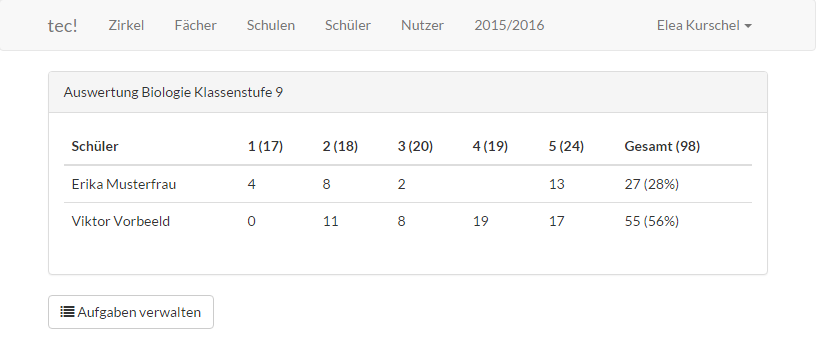
\includegraphics[scale=.50]{bilder/Protokoll_Auswertung.png}
	\caption{Beispiel Auswertung Zirkel}
	%\label{abb:beispiel}
\end{figure}

Außerdem kann man nun unter der Musterschule sehen, welche die aktiven Teilnehmer sind. Es sind nur Erika und Viktor, da sie im Gegensatz zu Max tatsächlich an einer Korrespondenz teilnehmen.

\begin{figure}[h]
	\centering
	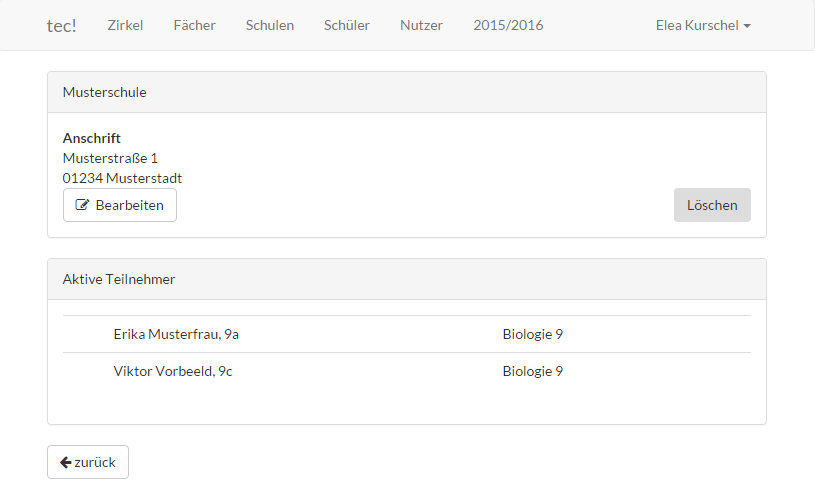
\includegraphics[scale=.50]{bilder/Protokoll_Schule.png}
	\caption{Beispiel Teilnehmer einer Schule}
	%\label{abb:beispiel}
\end{figure}

\chapter{Zusammenfassung}

\blindtext
\blindtext


% Glossar

\chapter*{Glossar}

\begin{description}
\item [JavaScript] Blindtext ist ein \LaTeX-Paket, welches es zu Demonstrationszwecken erlaubt, an beliebigen Stellen eines Dokumentes Fließtext ein zu setzen. Es handelt sich immer um den folgenden Text:
	
\item [MySQL] Blindtext ist ein \LaTeX-Paket, welches es zu Demonstrationszwecken erlaubt, an beliebigen Stellen eines Dokumentes Fließtext ein zu setzen. Es handelt sich immer um den folgenden Text:

\item [PHP] Blindtext ist ein \LaTeX-Paket, welches es zu Demonstrationszwecken erlaubt, an beliebigen Stellen eines Dokumentes Fließtext ein zu setzen.


\item [XAMPP] Blindtext ist ein \LaTeX-Paket, welches es zu Demonstrationszwecken erlaubt, an beliebigen Stellen eines Dokumentes Fließtext ein zu setzen.

\end{description}
\bibliography{litlist}
\bibliographystyle{amsalpha}
\begin{thebibliography}{999}

\bibitem{Xampp} \textsc{Apache Friends}: \textit{XAMPP}\\
			{\small Stand: ?, Zugriff: ?,} \\
			\url{https://www.apachefriends.org/de/index.html}
			
\bibitem{Apache} \textsc{Behlendorf}, B.; \textsc{Fielding}, R.; \textsc{Hartill}, R.; \textsc{Robinson}, D.; \textsc{Skolnick}, C.; \textsc{Terbush}, R.; \textsc{Thau}, R.; \textsc{Wilson}, A.; \textit{Apache HTTP SERVER PROJECT}\\
			{\small Stand: ?, Zugriff: 21.03.2016,} \\
			\url{https://httpd.apache.org/}
			
\bibitem{Eclipse} \textsc{Eclipse Foundation}: \textit{Eclipse}\\
			{\small Stand: ?, Zugriff: 21.03.2016,} \\
			\url{https://eclipse.org/}

\bibitem{Font} \textsc{Gandy}, Dave: \textit{Font Awesome}\\
			{\small Stand: 15.03.2016, Zugriff: 21.03.2016,} \\
			\url{https://fortawesome.github.io/Font-Awesome/icons/}
			
\bibitem{Korrespondenzzirkel} \textsc{Kriester}, Ulf-Armin: \textit{Regionalzentrum Ostthüringen}\\
			{\small Stand: ?, Zugriff: 21.03.2016,} \\
			\url{http://www.regionalzentrumostthueringen.de/index.php}
			
\bibitem{MySql} \textsc{Oracle Corporation}: \textit{MySQL}\\
			{\small Stand: 19.03.1016, Zugriff: 21.03.2016,}\\
			\url{https://www.mysql.de/}

\bibitem{Bootstrap} \textsc{Otto}, Mark; \textsc{Thornton}, Jacob: \textit{Bootstrap, Framework mit HTTP, CSS und JAVASCRIPT}\\
			{\small Stand: 19.03.1016, Zugriff: 21.03.2016,}\\
			\url{http://holdirbootstrap.de/}
			
\bibitem{laravel} \textsc{Otwell}, Taylor: \textit{Laravel, php Framework}\\
			{\small Stand: ?, Zugriff: ?,} \\
			\url{https://laravel.com/}

\bibitem{LaTex Grundlagen} \textsc{Stein}, Sebastian: \textit{Eine kleine \LaTeX \  Einführung}\\
			{\small Stand: 10.01.2016, Zugriff: 21.03.2016,} \\
			\url{http://latex.hpfsc.de/content/latex_tutorial/grundlagen/}
		
\bibitem{github} \textsc{Wanstrath}, Chris.; \textsc{Hyett}, PJ.; \textsc{Preston-Werner}, Tom.:  \textit{Github}\\ 
			{\small Stand: 21.03.2016, Zugriff: 21.03.2016,}\\ 			
			\url{https://github.com/}			
			
%	Vorname, Nachname, (erscheinungsjahr), Titel(aus(/title)), 
%	Art(www.seite:stand: letze Änderung, url, (Zugriff: Datum, Uhrzeit).
\end{thebibliography}


\listoffigures
\listoftables

\chapter*{Nutzungserklärung}
Hiermit erklären wir uns einverstanden, dass die Dokumentation und das Projekt für
schulische Zwecke verwendet werden dürfen.
Wir gestatten, die Dokumentation und das Projekt auf der Website der Schule und zum
Tag der offenen Tür zu veröffentlichen.

\chapter*{Erklärung der eigenständigen Erstellung des Projektes}
Hiermit versichern wir, dass wir die Dokumentation und Projekt selbstständig verfasst und
keine anderen als die angegebenen Quellen und Hilfsmittel benutzt haben sowie das alle
Ausführungen, die den Quellen wörtlich oder sinngemäß entnommen wurden, als solche
gekennzeichnet wurden.

\end{document}
